% !TEX program = xelatex
\documentclass[
  10pt,
  twoside,
  openany,
  b5paper, % 以上均为 ctexbook 提供的文类选项
  colorscheme = basic, % 请根据需要选择或定制配色方案
]{qyxf-book}
\usepackage{pdfpages}
\usepackage[contents = 钱院学辅, scale = 15, color = black, angle = 50, opacity = .10]{background}
\includepdfset{pagecommand={\thispagestyle{plain}}}

\title{数学物理方程笔记}
\subtitle{Notes on Equations of Mathematical Physics}  % 可选
\author{越杰91张玉辰}
\date{2021 年 1 月 8 日}
%\typo{AlphaGo}  % 排版人员信息,选填

% 定制元信息
\org{\Large\textit{钱学森书院学业辅导中心}\\\textsc{Qian Xuesen College Academic Counseling Center}}
\footorg{\textsc{Qian Yuan Xue Fu}}
\cover{
	\begin{tikzpicture}[remember picture, overlay]
		\begin{pgfonlayer}{background}
			\node at ($(current page.east)+(0in,0in)$){
				
\includegraphics[width=.8\textwidth]{cover.png} };
		\end{pgfonlayer}
	\end{tikzpicture}
}
\license{}  % 清空许可证信息

% 调整封面标题大小
\renewcommand{\titlefont}{\Huge\bfseries}
\renewcommand{\subtitlefont}{\LARGE\itshape}

\begin{document}

\maketitle

\chapter*{前言}
\thispagestyle{empty}

数学物理方程,简称“数理方程”,是多数工科专业同学必修的课程,它通过对一些具有典型意义的实际模型的深入剖析,阐明和讲述偏微分方程的基本理论、处理问题的典型技巧以及应用的物理背景,既是数学联系其他自然学科和技术领域最重要的桥梁之一,同时也为非数学类理工科专业的后继课程提供必要的数学工具,更重要的是对培养学生应用数学理论和方法解决实际问题的能力大有裨益。

2020-2021第一学期的数理方程课程安排在9-16周,因而课程内容未覆盖《数学物理方程(第2版)》的全部内容,笔者也是遵照代课老师讲解的主干内容整理得到如下知识结构,对于未涉及的部分有待其他同学进一步补充(由于笔者使用的“幕布”软件支持共享,欢迎同学们通过链接\url{https://share.mubu.com/doc/GUWy5o73ry}继续在“幕布”平台进行个人创作)。

笔者的“数理方程”课程由秦军林老师代课,秦老师采用的授课方式主要是板书,在授课过程中尤其注重公式的推导证明与题目的解答推演,经常写满黑板。根据本人的观察和了解,许多同学通过拍照板书作为课堂笔记,但部分手写体不好辨认、不便联系多块黑板上的板书,在完成作业和复习的过程中如上问题给同学们带来了较大困扰。鉴于此,本人利用空闲时间整理了这份知识结构,一来通过整理知识体系加深了自己对知识的记忆与理解,二来便于为广大同学勾勒本课程的知识体系便于总结与复习。值得说明的是,在这份知识结构中,我略去了各项结论推导证明的过程,但读者应该着重回顾贝塞尔方程本征值问题的证明过程、格林公式的推导过程;对于诸如“叠加原理”、“特殊区域上的格林函数”等只是罗列了条目,没有写具体内容,原因在于这些内容或相对简单、或因题而异,读者可以寻找相关题目在练习中积累方法经验;对于分离变量法,本文着重介绍四大步骤,希望读者理论联系实践,在练习中增进理解。

笔者在学习“数理方程”时,往往会因解题过程的复杂而产生抵触情绪,同时又会出现因不熟悉公式定理导致做题效率低下的问题。然而在一段时间的学习后,本人逐渐意识到数学学习的魅力正是在于通过个人的不懈努力最终解决困难问题的过程,而当加深了对知识的记忆和理解后再加以练习,容易取得理论认识和实践熟练度相长的良性循环。由衷希望本文能够为广大同学的在此课程的学习提供切实帮助,如有任何意见或建议也可随时向“钱院学辅”提出,谢谢大家!


\rightline{——越杰91\ 张玉辰} 
\newpage
\setcounter{page}{1}

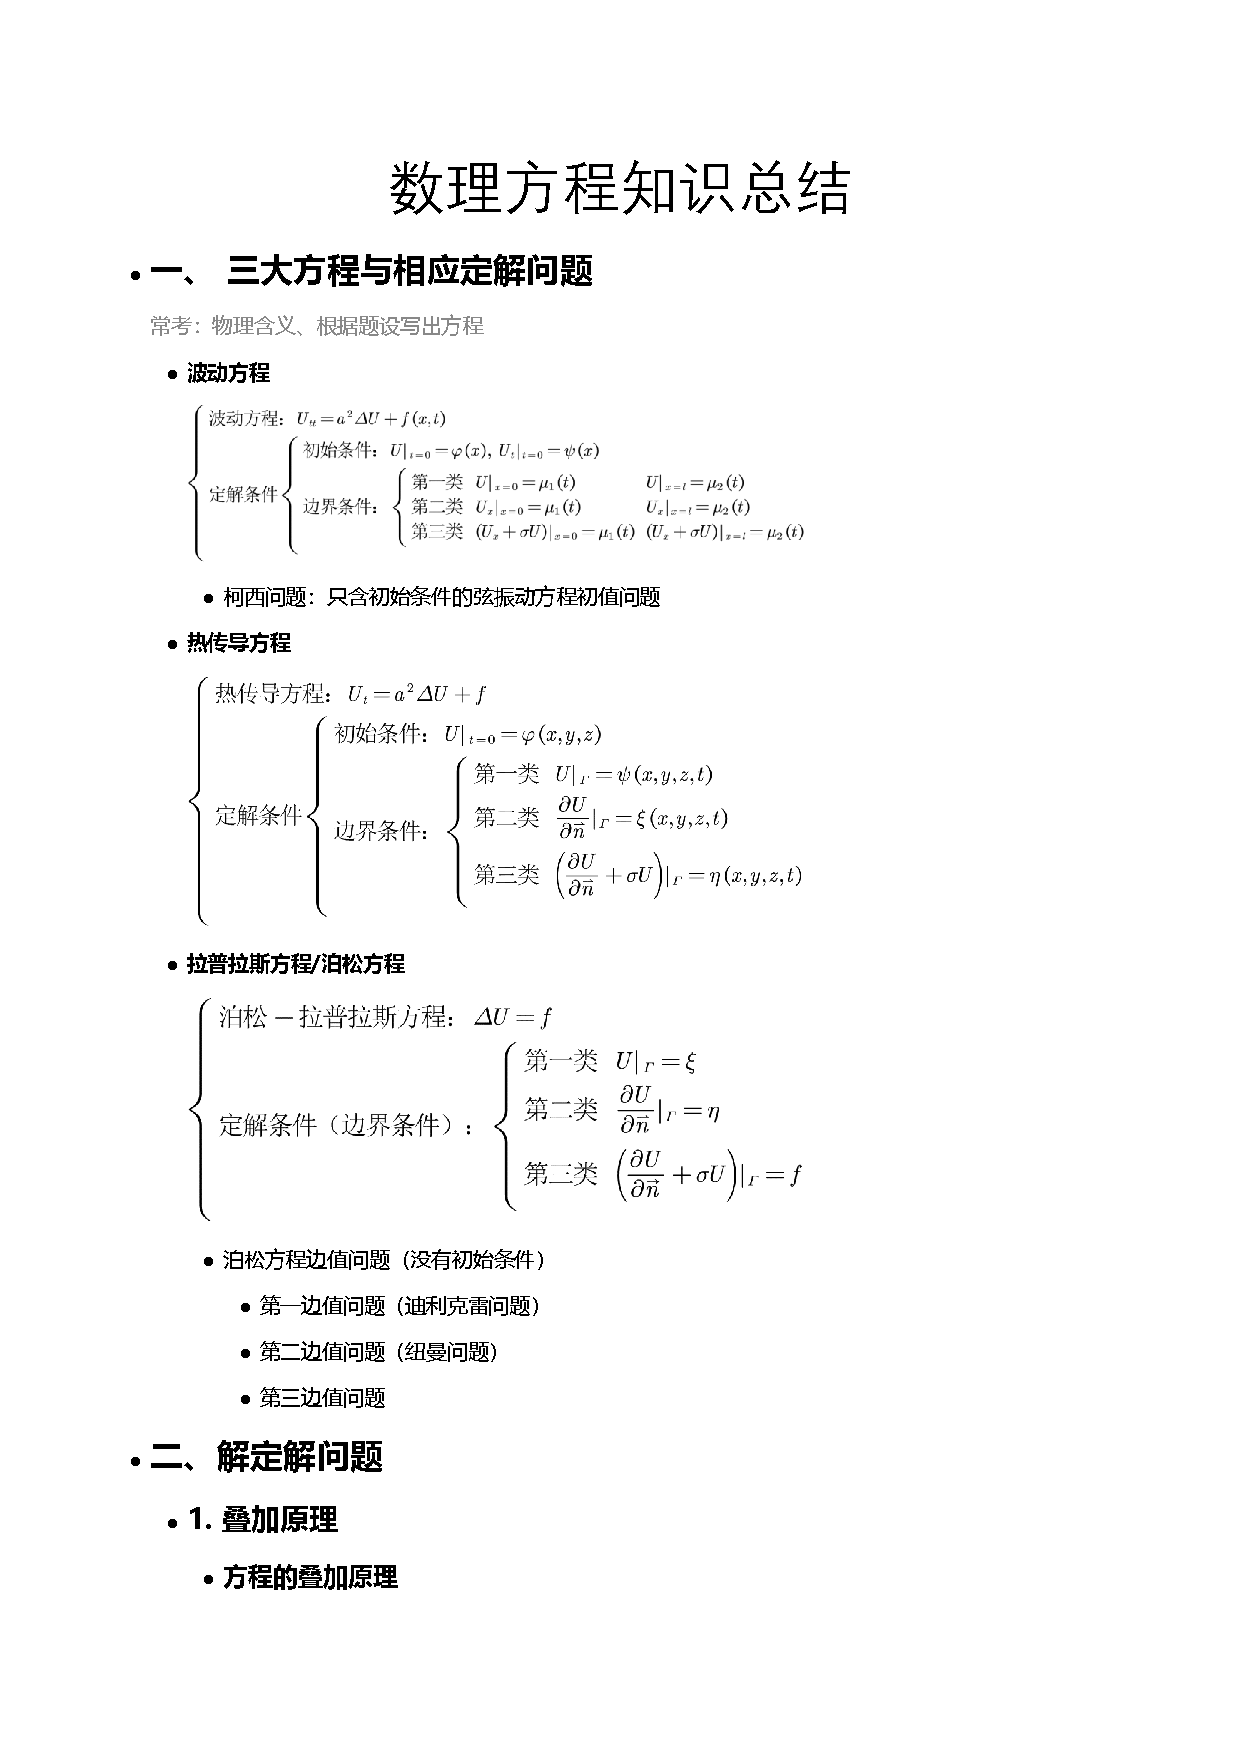
\includepdf[pages = - ]{content.pdf}


\includepdf[pagecommand = {\thispagestyle{empty}}, pages = - ]{lastpage.pdf}

\end{document}